%!TEX root =  main.tex


\section{Our approach}
In this section, we formally describe our \BertMWE approach.
We will start by formally describing our modelling framework in a probabilistic setting , 
and then introduce our approach for modeling the posterior distribution , 
and finally, produce the approximate inference procedure
and discuss some details on how it's implemented in deep transformer network.


\begin{figure}[tb]
    \centering
    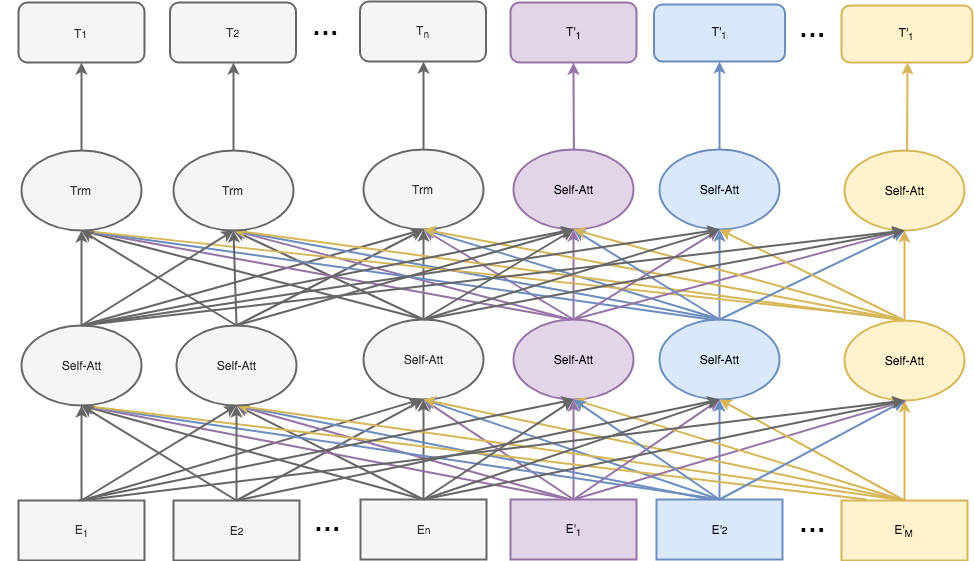
\includegraphics[width=0.95\linewidth]{fig/architecture.png}
    \vspace{20pt}
    \caption{\BertMWE architecture illustration. Grey nodes denotes the original self attention network. Nodes colored in purple, blue and yellow denotes the additional blocks corresponding to specific MWEs.}
    \vspace{10pt}
    \label{fig:variational}
\end{figure}


\subsection{Architecture overview}\label{sec:arch-overview}
In this work we assume that each input text instance are represented as a sequence of tokens $(w_1, ..., w_n)$,
and in addition, there are a set of candidate multi-world expressions $(w'_1, ..., w'_m)$, each corresponds to a span in the original token sequence, with starting index $(st_1, ..., st_m)$, and ending index $(end_1, ..., end_m)$. 

In typical self-attention network such as the original Bert model \cite{devlin2018bert}, the first step is to transform the input sequence into an unordered set, 
and the original position information is captured using the position embedding mechanism \cite{vaswani2017attention}. which on a high level, can be described as representing the input into the form of a permutation invariant set $\{u_1, ..., u_n\}$, where each element $u_i=(w_i, pos_i)$ include both the token $w_i$ and its position $pos_i$, in this case it index in the original sequence $i$.

As illustrated in \autoref{fig:variational}, each element in the input then go through the embedding layer and represented as a set of permutation invariant embeddings vectors $\{E_1, ..., E_n\}$, 
\cite{vaswani2017attention}
and then go through certain numbers of inter-connected self-attention layers, and finally go   to be mapped to the final output layers
$\{T_1, ..., T_n\}$
through some final layers of transformation the's suitable for the specific tasks at hand,  such as sequence labeling and classification \cite{devlin2018bert}.

In \BertMWE, we inject multiword expression into the network in an \textit{homogeneous} fashion: we insert the MWE as additional elements into the input, while the model architecture for processing these input stay the same. 

Specifically, given a set of candidate multi-world expressions $(w'_1, ..., w'_m)$, 
we will similarly transform them into a set of candidate multi-world expressions $(u'_1, ..., u'_m)$, where each element $u_i=(w'_i, pos'_i)$ include the mwe $w'_i$ and its location, which is derived as a function of the span location $f(st_i, end_i)$ in the original sequence $pos'_i$ \footnote{in this work we use the simple average function $f(st_i, end_i) = \lceil \frac{st_i, end_i}{2} \rceil $}.
Then, analagously, we embed the multi-world expressions $(u'_1, ..., u'_m)$ into embeddings vectors $\{E'_1, ..., E'_m\}$.
As shown in \autoref{fig:variational}, the embedding vectors $\{E'_1, ..., E'_m\}$ are concated  with the original vectors, and the newly concatenated set vectors 
$\{E_1, ..., E_n, E'_1, ..., E'_m\}$ are in the exact same form of the original input and fed to the exact same model as before.

The challenge with this approach, however, is that we don't know how many of the candidate MWEs are truly non-compositional and are important for capturing the meaning of the text and best support downstream prediction tasks:
Simply adding all of them into the original tokens' embedding would potentially introduce large amount of noise to the data and obfuscate the original inputs. Blindly ignoring some candidates might miss important non-compositionality information.
we need a way to distinguish good from the bad, and dynamically infer the non-compositionality, along with the set of parameters contained in the deep self-attention networks architecture.


We formualte this using a principled bayesian probabilistic framework. 
Given a dataset $\mathcalD$ containing a set of $N$ observations of tuples $(x,y)$,  $x$ is the input text and $y$ is the target labels of interest ,
if we use  $m_{MWE}$ to denote the model to select from the set of candidate multi-world expressions the true non-composable MWEs to be included in the final model, and 
$m_{Bert}$ to denote the original self attention network that predict the target output from the inputs, the task can then be formally described as a posterior probability inference over the space of all possible models $m_{MWE} \in M_{MWE}, m_{Bert} \in M_{Bert}$, as the following
\begin{align*}
\small
\begin{split}
    P(m_{MWE}, m_{Bert} | \mathcalD) = \frac{  P( \mathcalD | m_{MWE}, m_{Bert} ) P(m_{MWE}, m_{Bert})  }{ \int \int P( \mathcalD | m_{MWE}, m_{Bert} ) P(m_{MWE}, m_{Bert}) }\\
\end{split}
\end{align*}


\subsection{variational parameterization}\label{sec:var-param}


\begin{figure}[tb]
    \centering
    \includegraphics[width=\linewidth]{fig/variational_inference.png}
    \vspace{20pt}
    \caption{Graphical model representation for the proposed variational distribution. Plates represent replications over each possible MWEs and each data instances. Empty nodes denotes the latent variables and solid nodes denotes observed data. The latent variables are instantiated and resulted in a neural network, into which the input is passed to and the output is collected. }
    %\vspace{10pt}
    \label{fig:variational}
\end{figure}


The above inference problem is intractable because of the computing the true posterior distribution involves integrals over all possible model spaces which is computationally intractable. 
Instead, we follow  variational inference principle \cite{} to approximate the model posterior with a family of variational distribution $\mathcal{Q}$ over the models, and the goal is to find find a specific distribution $q(m_{MWE}, m_{Bert}) \in \mathcal{Q}$ that are closest to the exact posterior distribution $P(m_{MWE}, m_{Bert} | \mathcalD)$.
We will first describe our choice of the variational family $\mathcal{Q}$, and then continue to specify the variantional inference procedure.


The goal of the \BertMWE is to learn to capture both the individual non-compositionality from the MWEs while fully utilize the modeling power of the deep self-attention network. To that end we propose the a procedure to parameterize our distribution family $\mathcal{Q}$, 
as a probabilistic generative process. 
The basic idea is to view the output target as a mixture of possible models applied to the given input x, 
while including the selection of MWEs as integrated part of the network architecture.
The decision for the inclusion of MwEs is make in a hierarchical manner by a global factor controlling the joint quality of the MWE architecture as well as independent qualities for each MWE.

Specifically, we assuming the network is described by of mean parameter matrixes $W$, and a prior distribution for Bernoulli variables, parameterized by $\Pi$ and $\p_i$ where $i$ range across of the vocabulary of all possible MWEs $v$. The generation process can be described as
\begin{enumerate}
    \item Initialize the network $\Theta$ to skip any MWE in the input by multiplying correspondings parameters in $W$ by zero
    \item Choose global mwe decision variable 
        $b \sim \mbox{Bernoulli}(\Pi)$
    \item{for each MWE in the vocabulary $V$}
    \begin{enumerate}
        \item draw a decision variable $\beta_i \sim \mbox{Bernoulli}(\pi_i)$ for that MWE 
        \item{unmute the MWE parameters in model $\Theta$ only if $s_{j}=1$ and $s_{j}=1$}
    \end{enumerate}
    \item{Choose token $y_{di} \sim \mbox{Mult}(p(x))$}
\end{enumerate}


We can also represent \BertMWE model using the the probabilistic graphical notation, as shown in \autoref{fig:variational}. 
On the top levels are parameters $\Pi$ and $\pi_i, i \in V$, $W$, which are corpus level parameters. Then for each of the $N$ training instance, the set of Bernoulli latent variables
$B$, $\beta_i, i\in v$ are drawn, from which we obtain a specific instantiation of the neural network with parameters $\Theta$. And finally, we pass the input $x$ through the neural network, and outcome of the neural network is generated.


If we denote $\Theta = \{\Theta_{Bert-MWE}, B, \{\beta_i | i \in V\} \vert x,y \in \mathcalD \}$ as the latent variable for the model configurations for each instance in the data, and $Q(\Theta | W, \Pi, \{\pi_i | i \in V\})$ it variational distribution given  
the Bernoulli parameters $\Pi$ and $\pi_i$, and the mean parameter matrices $W$,
The expected log likelihood for the observed data $\mathcalD$ over all the possible configurations can be specified as 
\begin{align}
& \mathbb{E}_{\Theta \sim Q} \log P (\mathcalD | \Theta) \nonumber\\ 
= & \sum_{x, y \in \mathcalD} \int_{\Theta} \log p(y \vert f^{\Theta}(x)) Q(\Theta | W, \Pi, \{\pi_i | i \in V\}) \nonumber\\ 
= & \sum_{x, y \in \mathcalD} \int_B \int_{\beta_i}\int_{\Theta_{Bert-MWE}} \log ( p(B | \Pi) \prod_i^{V} p(\beta_i | \pi_i) \nonumber\\ 
& \quad \quad \quad \quad p(\Theta_{Bert-MWE} \vert W, B, \{\beta_i, i \in V\}) \nonumber\\ 
& \quad \quad \quad \quad p(y \vert f^{\Theta_{Bert-MWE}}(x)) )
\label{eq:exp}
\end{align}

where the conditional distribution 
$p(B | \Pi)$, $p(\beta_i | \oi), i\in v$ are given by the Bernoulli distribution with $\Pi$ and $\pi_i, i\in v$ being the mean parameter, 
$p(\Theta_{Bert-MWE} \vert W, B, \{\beta_i, i \in V\})$ specifies the outcome of zeroing and unzeroing the networks weights $W$ according to the Bernoulli variable $B, \{\beta_i, i \in V\})$ as described by the generative process above,
and finally $p(y \vert f^{\Theta}(x))$ describes the predicted probability of the network as parameterized by $\Theta$ for the target output $y$ given input text $x$. 




Following the variantional inference principle, our goal is then to optimize the parameters for the variational distribution to make it as close to the true model posterior as possible. Specifically, we aim to optimize the the evidence lower bound (ELBO) for the marginal log likelihood of the data $\log P( \mathcalD )$: 
\begin{align}
    &\log P( \mathcalD ) \nonumber\\
    = & \int_{M_{Bert}} \int_{M_{Bert}} \log P( \mathcalD | m_{MWE}, m_{Bert} ) \nonumber\\
    \geq& \mathbb{E}_{\Theta \sim Q} \log P (\mathcalD | \Theta) - D_{KL}(Q( \Theta) ||\mathcal{P}( \Theta)) \nonumber\\
    = & \mathcal{L}_{Bernoulli} (W, B, \{\beta_i, i \in V\}) \label{eq:elbo0}
\end{align}

where $\mathbb{E}_{\Theta \sim Q} (P (\mathcalD | \Theta) )$ is the expectation of the conditional likelihood under the variational distribution as described in \autoref{eq:exp}, and the KL divergence between the variational distribution and the prior distribution of the model parameters $\mathcal{P}(\Theta)$, $D_{KL}(Q( \Theta) ||\mathcal{P}( \Theta))$ can be approximated  as in \cite{gal2016uncertainty}.
%
%, we omit this term in practise and focus on optimizing the likelihood term  $\mathbb{E}_{\Theta \sim Q} (P (\mathcalD | \Theta) )$.


%Following the variational interpretation, dropout is seen as an approximating distribution $q_\theta(\bo)$ to the posterior in a Bayesian neural network with a set of random weight matrices $\bo = \{\W_l\}_{l=1}^L$ with $L$ layers and $\theta$ the set of variational parameters. 
% Assume that the weight matrices can be written as $\bo = g(\theta, \bepsilon)$ with $\epsilon$ a random variable that does not depend on $\theta$.
%The optimisation objective that follows from the variational interpretation can be written as:
